\documentclass[10pt]{article}

\usepackage[utf8x]{inputenc}
\usepackage[T1]{fontenc}
\usepackage{amsfonts,amsmath,amssymb,amsthm,booktabs,color,graphicx}
\usepackage[ruled,vlined,linesnumbered]{algorithm2e}
\usepackage{enumitem}

\title{String Processing Algorithms 2015 - Week 1 Exercises}
\author{Rodion Efremov}
\date{\today}

\begin{document}
\maketitle

\section*{Exercise 1}
\color{blue} The worst case time complexity of the standard quicksort algorithm is $\Omega(n^2)$, but by a suitable pivot selection one can achieve $\mathcal{O}(n \log n)$ time. Explain how to achieve
\begin{enumerate}[label=(\alph*)]
\item average time complexity $\mathcal{O}(n \log n)$
\item expected time complexity $\mathcal{O}(n \log n)$
\item worst case time complexity $\mathcal{O}(n \log n)$.
\end{enumerate}
\color{black}

\subsection*{Solution}
\subsubsection*{(a)} Whenever we are dealing with an \textbf{average} time complexity, the assumption is that the algorithm is \textbf{not} random. Basically, we assume that every input is equally likely and we compute the average time complexity simply by summing all running times over all inputs and by dividing by the number of inputs; the same way as an average is computed.

In order to achieve an average time complexity $\mathcal{O}(n \log n)$ for the quicksort, whenever calling the actual quicksort routine with a particular range to sort, we could program it to choose, say, three pivots: one from the beginning of the input range, one from the end of the input range and one from the middle of the input range. After that, use the pivot that is second largest.

\subsubsection*{(b)} Whenever talking about \textbf{expected} time complexity, the assumption is that the algorithm is \textbf{randomized}, i.e, it relies on a pseudorandom number generator in order to make decisions.

We can guarantee an expected time complexity $\mathcal{O}(n \log n)$ if we choose pivot/pivots randomly.

\subsubsection*{(c)} In order to quarantee the \textbf{worst case} time complexity $\mathcal{O}(n \log n)$ for a quicksort implementation, I see no other possibility but using \textbf{Introsort}: use a quicksort with arbitrary pivot selection scheme, but keep track how deep in the recursion we get; if we exceed some precomputed depth, sort the range using \textbf{heapsort}, which guarantees the worst case time complexity of $\mathcal{O}(n \log n)$.

\section*{Exercise 2}
\color{blue} A full binary tree is a binary tree where every node is either a leaf or has two children. Show that every full binary tree with $n$ leaves has exactly $2n - 1$ nodes. \textit{Hint: Use induction.}
\color{black}

\subsection*{Solution}
\textbf{The base case:} Suppose $n = 1$. The only possibility is that the leaf node is, in fact, the only node of the tree: $2n - 1 = 2 - 1 = 1$. \\
Now, the formula tells us that adding a new node (call it $u$) to the tree (such that the tree remains a full binary tree) introduces two nodes: $u$ itself and some node (call it $v$) that makes sure that the binary tree remains full. We have two cases:
\begin{enumerate}[label=(\Roman*)]
\item Adding the new node to a leaf of the tree.
\item Replacing a node with a new node.
\end{enumerate}

\subsubsection*{Case I} Choose a leaf node $x$ of the tree. Attach $u$ to it. Now the tree is not full because $x$ has only one child ($u$). In order to fix the full binary tree invariant, we add $v$ as the other child of $x$. Now the tree is a full binary tree. Note that $x$ is no longer a leaf node, but the tree received two new leaf nodes, so the amount of leaves increased by one, and the amount of all nodes of the tree increased by two nodes.
\begin{center}
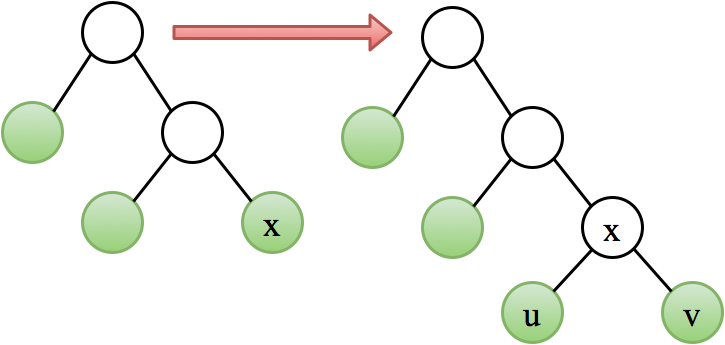
\includegraphics[scale=0.3]{FullBinaryTreeCaseI}
\end{center}

\subsubsection*{Case II} Choose an arbitrary node $x$. Substitute $x$ with $u$ and attach $x$ as one of the children of $u$. At this point $u$ has only one child; add $v$ as the other child, which makes the binary tree full. The amount of leaves increased by one and amount of nodes increased by two as expected.
\begin{center}
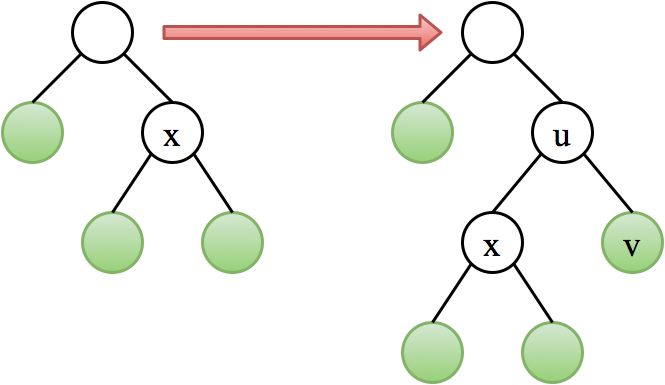
\includegraphics[scale=0.3]{FullBinaryTreeCaseII}
\end{center}
Now by induction principle, the proof is complete.

\section*{Exercise 3}
\color{blue} Transform the following nondeterministic finite automaton into a deterministic finite automaton.
\begin{center}
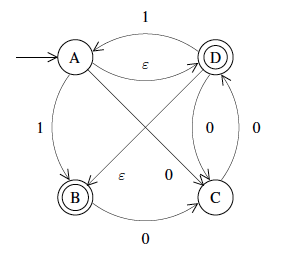
\includegraphics[scale=0.7]{Exercise3NFA}
\end{center}
\color{black}
\subsection*{Solution}
The initial state is $A$, so in the result DFA the initial state is $E(\{ A \}) = \{ A, B, D \}$.
\subsubsection*{$\{A, B, D\}$}
\begin{align*}
\delta'( \{ A, B, D \}, 0 ) &= E( \{ C \} ) = \{ C \} \\
\delta'( \{ A, B, D \}, 1 ) &= E( \{ A, B \}) = \{ A, B, D \}
\end{align*}
\subsubsection*{$\{ C \}$}
\begin{align*}
\delta'( \{ C \}, 0 ) &= E( \{ D \} ) = \{ B, D \} \\
\delta'( \{ C \}, 1 ) &= E( \emptyset ) = \emptyset
\end{align*}
\subsubsection*{$\{ B, D \}$}
\begin{align*}
\delta'( \{ B, D \}, 0 ) &= E( \{ C \} ) = \{ C \} \\
\delta'( \{ B, D \}, 1 ) &= E( \{ A \} ) = \{ A, B, D \}
\end{align*}

\noindent The resulting DFA is 
\begin{center}
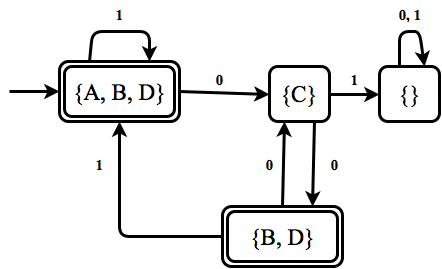
\includegraphics[scale=0.5]{Exercise3DFA}
\end{center}
\end{document}